\documentclass[11pt,oneside,final]{memoir}

\usepackage{soul}
\usepackage[cmyk]{xcolor}

\usepackage[pdftex]{graphicx}
\graphicspath{{./src-images/}}
\usepackage{eso-pic}

%% 5.25in x 8in
%% 133.4mm x 203.2mm

\usepackage{geometry}
\geometry{
paperwidth=5.25in,
paperheight=8in,
nohead,
nofoot,
margin=0pt
}
\setlength{\stockwidth}{5.25in}
\setlength{\stockheight}{8in}

\usepackage{fontspec}
\setmainfont[Ligatures = TeX]{Shaker 2 Light}

\newfontfamily\titleFont[Ligatures = TeX]{Shaker 2 Light}
\newfontfamily\subtitleFont[Ligatures = TeX]{Shaker 2 Light}
\newfontfamily\authorFont[Ligatures = TeX]{Shaker 2 Regular}

\sodef\soTitle{}{.1em}{.5em plus.1em}{.1em plus.1em minus.1em}

\pagestyle{empty}

\setlength{\parindent}{0pt}

\begin{document}
%
\centering%
%
\begin{minipage}[c][146mm][c]{\paperwidth}%
\centering%
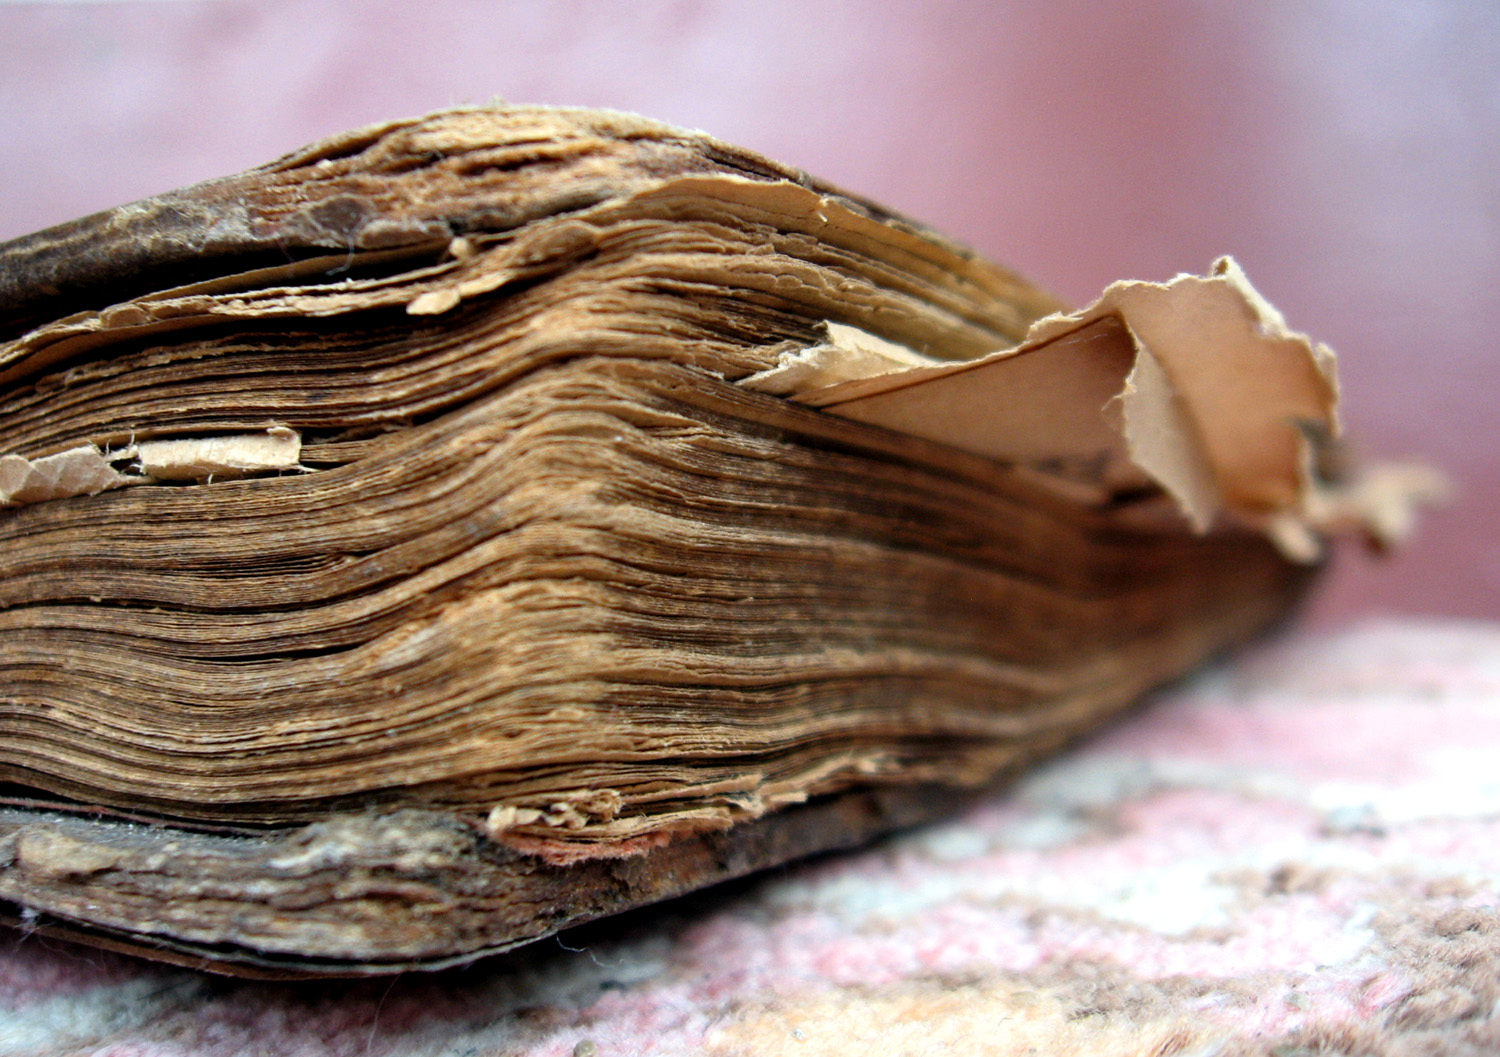
\includegraphics[height=146mm,keepaspectratio]{very_old_book_by_blue_bullet_CMYK.jpg}%
\end{minipage}

\vspace*{13mm}

{\titleFont\Huge\MakeUppercase{\soTitle{The Skeleton of a Book}}}

\vspace*{\baselineskip}

{\subtitleFont\Large an example of book design with \LaTeX}

\vfill

{\authorFont\Large \MakeUppercase{Unknown Author}}

\vspace*{12mm}

\end{document}
